\section{DebugIT - Ontology-mediated layered Data Integration for real-time Antibiotics Resistance Surveillance}

The DebugIT project is a good reference for analyzing how medical data integration can be done though this project didn't use a dataspace approach but an ontology-mediated \cite{WurstDiss, DBLP:books/dp/LeserN2006} approach. DebugIT stands for ``Detecting and Eleminating Bacteria Using Information Technology'' and its main goal is to provide a platform for high-throughput analysis of distributed clinical data as a response to the spread of antibiotic resistance of infectious pathogens in European hospitals\cite{UniFreiburgDebugITInfo}. 
The team of the DebugIT project released the architecture of their system in \cite{DBLP:conf/swat4ls/SchoberCDEDJTPLB14}.
In that paper it is stated, that the system uses an ontology-based approach for allowing antibiotics resistance data semantically and geographically interoperable. This makes it possible to integrate distributed clinical data EU-wide in real-time for monitoring antibiotic resistance. As well, the system is structured in four tiers and works in a service oriented manner (SOA). Figure \ref{DebugITArchitectureFigure} shows the layered architecture of the DebugIT's system:
\begin{figure}[H]
	\begin{center}
		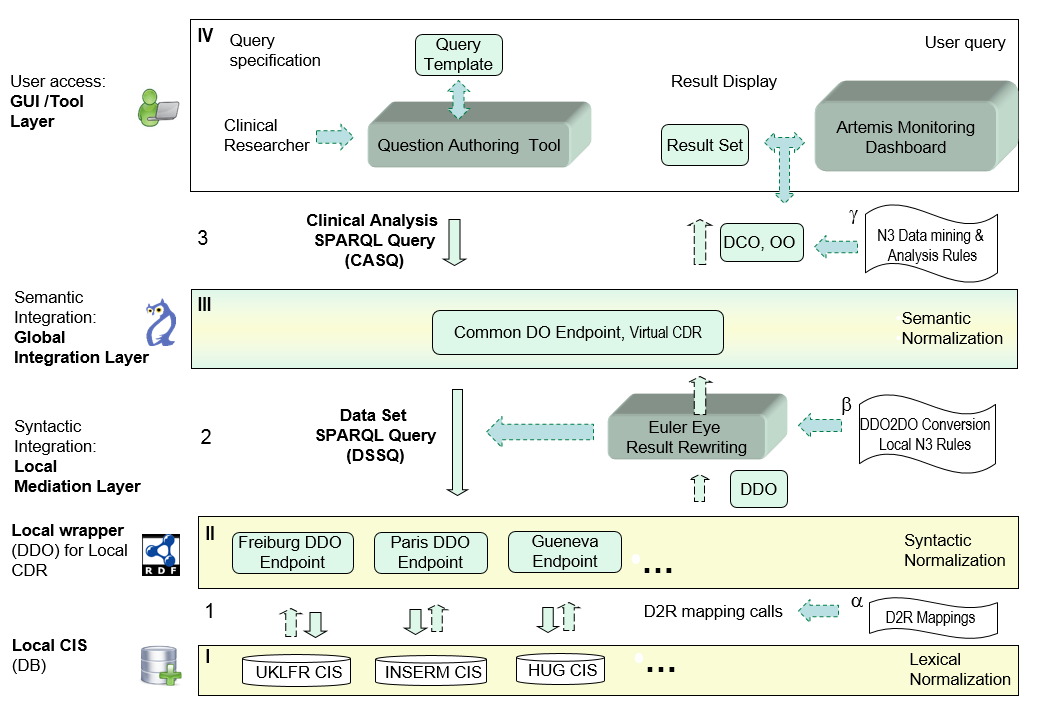
\includegraphics[width=0.75\textwidth]{figures/DebugIT-Ontology-mediated-layered-Data-Integration-architecture.png}
	\end{center}
	\caption{The layered mediator architecture of the DebugIT project}
	\label{DebugITArchitectureFigure}
\end{figure}

Altogether there are 3 data representation layers marked with the Roman Numerals I-III. The query flow between the data layers is specified with 1-3 and the corresponding mappings are given with the Greek letters \textalpha , \textbeta  and \textgamma .

On the first integration layer (I) relational data are lexical normalized by the use of mappings of medical terminology and morphosemantic mapping employed by the Averbis Morphosaurus software\cite{DaumkeDiss}. Ambiguities can be enriched with ontological expressions (formulated in OWL) on the integration layers II and III. The layer II works with RDF data, wherefore relational data from the layer I is transformed to RDF through D2R mapping calls \footnote{http://d2rq.org/} on the first mediation layer (1). On the second integration layer information about the data and their corresponding vocabulary is stored in Data Definition Ontologies (DDOs) \cite{DebugITDDO}. A DDO bridges a local data model and a semi-formal data model on the local mediation layer for integrating syntactic data and provides an Extract, Transform, Load (ETL)-process \footnote{DBLP:books/dp/LeserN2006} for the next integration layer. For each Clinical Data Repository (CDR) such a DDO is locally created. 

Layer II contains also a SPARQL endpoint, for allowing Layer III to query its data. These queries are specified through Data Set SPARQL Query (DSSQ). 
On the second mediation layer (2) the local DDO data is bind to the global DebugIT Core Ontology (DCO) \cite{Schober_developingdco:}, the data representation of layer III. The corresponding mapping (2) is done through DDO2DCO using the N3 language \footnote{http://www.w3.org/TeamSubmission/n3/} and Simple Knowledge Organization Structure (SKOS) mappings \footnote{http://www.w3.org/TR/2009/REC-skos-reference-20090818/}. The binding is done through the Euler Eye Reasoner \footnote{http://eulersharp.sourceforge.net/}.

Data layer III represents a virtual Clinical Data Repository (vCDR), which joins the local Clinical Information Systems (CISs). Through the virtualisation data of all CIS can be globally queried and privacy issues can properly be handled.
Also on layer III clinical analyses can be performed over Clinical Analysis SPARQL Queries (CASQ (3)). On the last layer (IV) a user or a monitoring tool can integratively query distributed clinical data.

Summarizing it, the mapping is performed iteratively in a stack-like manner:
The first mapping \textalpha (D2R mappings) transforms the relational database layer (I) to the RDF representation layer (II). The next mapping \textbeta (N3 and SKOS) transforms the RDF layer II to the Domain Ontology (OO) layer III, where the data is globally queryable as CASQ over mapping \textgamma (DCO and OO).  

\uline{Advantages and disadvantages:} Query complexity and lesser source transparency are known disadvantages of a wrapper-mediator architecture. As a comprising system would need to cover veterinary resistance occurrence, the system can be still seen as limited. 

\uline{Key advantages:}
\begin{itemize}
	\item The DebugIT monitoring tools access hospital data in real-time, hence allowing early trend discovery and opportunities for early interventions. Most of the other existing monitoring systems have a low timely resolution in reverse.
	\item DebugIT is not limited to a certain selected set of bacteria or sampling methods, but potentially includes all bacteria and strains as found in the hospital data that can be mapped to a DCO/Uniprot taxonomity.
	\item DebugIT stores data in a re-usable, semantically formal and traceable way.
\end{itemize}